\documentclass[twoside]{article}
\input{ISC18-english.sty}
%%%%%%%%%%%%%%%%%%%%%%%%%%%%  Make sure to compile twice for proper cross-references. %%%%%%%%%%%%%%%%%%%%%%%
%%%%%%% For proper display of references, compile the document twice. %%%%%%%%%%%%%%%%%%%%% 
%%%%%%%%%%%%%%% If using TeX Live, compile using pdflatex command %%%%%%%%%%%%%%%%%%%%%%%
\begin{document}
\thispagestyle{empty}
%%%%%%%%%%%%%%%%% Article title header  %%%%%%%%%%%%%%%%%%%%
\fancyhead[LE]{Enhancing Decision Tree Learning via Conditional Cumulative Residual Entropy}
%%%%%%%%%%%%%%%%% Article authors header   %%%%%%%%%%%%%%%%%%%%
\fancyhead[RO]{S. Abolhosseini, M.Khorashadizadeh }
\begin{center}
{
\includegraphics [height=25mm, width=150.3mm] {Images/isc18E}} \\
\vspace*{-1.8cm}
%\begin{center}
%\color{blue} 
%{\hspace{0.1cm}\rule{\textwidth}{1mm}}\\
%\end{center}
\vspace*{4cm}
%%%%%%%%%%%%%%%%% Article title  %%%%%%%%%%%%%%%%%%%%
{\Large \bf Enhancing Decision Tree Learning via Conditional Cumulative Residual Entropy: A Framework for Continuous Variables }\\
%%%%%%%%%%%%%%%%% Article authors and affiliations %%%%%%%%%%%%%%%%%%%%
{\bf
Somayeh Abolhosseini$^1$, Mohammad Khorashadizadeh  \footnote[2]{{\bf Corresponding Author:} {\tt }} \\
$^1$,$^2$Department of Statistics, University of Birjand, Birjand, Iran  \\
%$^2$Second Author's Affiliation
}
\end{center}
\rule{\textwidth}{0.2mm}\\
%%%%%%%%%%%%%%%%% Article abstract  %%%%%%%%%%%%%%%%%%%%
\noindent{\bf Abstract:}\\
%In writing the abstract, the main findings of the article should be expressed in a descriptive, concise, and useful manner. For this purpose, the abstract should not be less than 3 and more than 10 lines. Note that in the abstract, unusual abbreviations and formulas should be avoided as much as possible. Also, no reference numbers should be included.
% 
Conventional decision tree algorithms struggle with continuous variables, often causing information loss through discretization. This paper proposes a novel framework using Conditional Cumulative Residual Entropy (CCRE) to directly handle continuous inputs and outputs. Unlike traditional entropy measures, CCRE provides a more nuanced uncertainty measure for continuous distributions. The theoretical framework for the splitting criterion is derived, and its effectiveness is shown across regression and classification tasks. Empirical evaluations indicate that this approach eliminates discretization biases and yields superior predictive performance compared to baseline methods. The results highlight CCRE's potential as a powerful tool for tree-based learning, contributing significantly to data mining and machine learning.\\
\noindent{\bf Keywords:} 
Conditional Cumulative Residual Entropy, Decision tree, Machin learning \\
\noindent{\bf Mathematics Subject Classification (2010):} $\rm 99X99$, $\rm 99X99$, $\rm 99X99$. \\
\hspace{1cm}\rule{\textwidth}{0.2mm}\\
%%%%%%%%%%%%%%
\section{Introduction}
In the field of machine learning and data mining, datasets generally consist of discrete input and output data, continuous input and output data, or combinations thereof. This diversity of data types presents various challenges in the design and application of learning algorithms. Decision trees are an effective method for classification and regression tasks, applicable to both discrete and continuous data. However, many decision tree algorithms are originally designed for discrete data, facing limitations when dealing with continuous variables. These limitations often necessitate discretization, which can lead to significant loss of valuable information. Abolhosseini et al. (2024) introduced an algorithm that uses cumulative residual entropy to improve decision tree methods, primarily focusing on datasets with discrete inputs and outputs. In contrast, this article specifically addresses datasets with continuous inputs and outputs, proposing a novel decision tree algorithm based on conditional cumulative residual entropy. This algorithm effectively manages continuous data without the need for discretization. The proposed algorithm demonstrates competitive performance against conventional and advanced methods in both regression and classification tasks, offering a promising alternative for handling complex and continuous data. 
\section{CCRDT algorithm}
In the context of a scientific study, consider the target variable along with the features and the associated training dataset, which consists of n observations
\[
\begin{bmatrix}
y_1 & x_{11} & x_{21} & \cdots & x_{k1} \\
y_2 & x_{12} & x_{22} & \cdots & x_{k2} \\
\vdots & \vdots & \vdots & \ddots & \vdots \\
y_n & x_{1n} & x_{2n} & \cdots & x_{kn}
\end{bmatrix}
\]
Furthermore, let us consider that X and Y are continuous random variables. In the newly proposed decision tree algorithm, referred to as CCRDT, the information gain criterion is determined using the CCRE in the following manner: 

Information gain for feature \(X_i\) is defined as:
\begin{equation}\label{2}
InformationGain(X_i) = CRE(Y) - CRE(Y|X_i); \qquad i = 1, \dots, k.
\end{equation}

where $CRE(Y) = -\sum_{i=1}^{n}P(Y\geq y_{i}) \log P(Y\geq y_{i})(y_{i}-y_{i-1})  $ is the cumulative residual entropy of the target variable in the training data set, and \(\text{CRE}(Y|X_i)\) is the conditional cumulative residual entropy, calculated as follows for every \(X_i\):
\begin{equation}\label{3}
\mathrm{CRE}(Y|X_i) = -\sum_{t=1}^{n}\sum_{j=1}^{n} \dfrac{\#(Y>y_t,\, X_i = x_{ij})}{n} \log \dfrac{\#(Y>y_t,\, X_i = x_{ij})}{\#(X_i = x_{ij})} (y_t - y_{t-1})
\end{equation}

The process of constructing a decision tree involves several key steps:

\begin{enumerate}
    \item Calculate the conditional risk estimate (CRE) of the target variable, denoted as \(\widehat{\varepsilon(Y)}\), using equation (1).
    \item Determine the conditional CRE for each qualitative feature random variable through the estimator outlined in equation \eqref{3}.
    \item Assess the information gain associated with each feature by applying equation \eqref{2}.
    \item The feature that yields the highest information gain will be chosen as the splitting criterion at the tree's root. Subsequently, the training dataset will be divided based on the number of levels at the root, and the process from Steps 1 to 4 will be repeated until the final decision tree is fully developed.
\end{enumerate}
%%\section{ Comparisons and Application to real data sets }
%%Evaluating decision tree performance involves more than just predictive accuracy; computational efficiency and interpretability are also key. This study compares ID3 and CCRDT using accuracy, confusion matrix, F-score, and ROC curve. Random Forest, CCRDT, and CART are compared using MSE, RMSE, R-squared, and training time. Eight diverse datasets (e.g., Abalone, Concrete, Wine Quality, California Housing) were preprocessed and evaluated using cross-validation to ensure robustness and reduce overfitting. Finally, the proposed CCRDT algorithm is developed and applied to each dataset following outlined steps.
%%
%%\begin{table}[htbp]
%%\centering
%%\caption{Comparative analysis of evaluation criteria for CCRDT and ID3}
%%\begin{tabular}{|l|l|c|c|c|c|}
%%\hline
%%\multicolumn{2}{|c|}{Dataset name} & \multicolumn{4}{c|}{Evaluation criteria} \\
%%\hline
%%\multicolumn{2}{|c|}{} & Accuracy & Precision & Recall & F1-score \\
%%\hline
%%Abalone & CCRDT & 0.76 & 0.80 & 0.68 & 0.74 \\
%%\hline
%%Abalone & ID3 & 0.73 & 0.73 & 0.74 & 0.74 \\
%%\hline
%%Concrete Compressive Strength & CCRDT & 0.82 & 0.78 & 0.85 & 0.81 \\
%%\hline
%%Concrete Compressive Strength & ID3 & 0.81 & 0.80 & 0.86 & 0.82 \\
%%\hline
%%Wine Quality & CCRDT & 0.53 & 0.53 & 0.99 & 0.70 \\
%%\hline
%%Wine Quality & ID3 & 0.72 & 0.70 & 0.73 & 0.71 \\
%%\hline
%%California Housing & CCRDT & 0.79 & 0.78 & 0.89 & 0.83 \\
%%\hline
%%California Housing & ID3 & 0.78 & 0.77 & 0.88 & 0.82 \\
%%\hline
%%Energy Efficiency & CCRDT & 0.99 & 0.97 & 1.00 & 0.99 \\
%%\hline
%%Energy Efficiency & ID3 & 0.98 & 0.50 & 1.00 & 0.68 \\
%%\hline
%%Airfoil Self-Noise & CCRDT & 0.76 & 0.72 & 0.89 & 0.80 \\
%%\hline
%%Airfoil Self-Noise & ID3 & 0.61 & 0.57 & 0.65 & 0.61 \\
%%\hline
%%Combined Cycle Power Plant & CCRDT & 0.93 & 0.98 & 0.90 & 0.94 \\
%%\hline
%%Combined Cycle Power Plant & ID3 & 0.93 & 0.98 & 0.90 & 0.94 \\
%%\hline
%%Life Expectancy (WHO) Fixed & CCRDT & 0.91 & 0.94 & 0.90 & 0.92 \\
%%\hline
%%Life Expectancy (WHO) Fixed & ID3 & 0.80 & 0.75 & 0.91 & 0.64 \\
%%\hline
%%\end{tabular}
%%\end{table}
%%\begin{table}[htbp]
%%\centering
%%\caption{Comparison between CCRDT, Random Forest and CART}
%%\begin{tabular}{|l|l|c|c|c|c|}
%%\hline
%%Dataset name & Type of Tree & MSE & RMSE & R-squared & Training time (Second) \\
%%\hline
%%Abalone & CCRDT & 1.07 & 1.03 & 0.30 & 2.19 \\
%%\hline
%%& Random Forest & 4.60 & 2.10 & 0.56 & 9.49 \\
%%\hline
%%& CART & 0.13 & 0.35 & 0.11 & 0.08 \\
%%\hline
%%Concrete Compressive Strength & CCRDT & 0.003 & 0.062 & 0.97 & 2.09 \\
%%\hline
%%& Random Forest & 0.36 & 0.56 & 0.88 & 0.94 \\
%%\hline
%%& CART & 0.11 & 0.34 & 0.51 & 0.02 \\
%%\hline
%%Wine Quality & CCRDT & 0.01 & 0.11 & 0.44 & 0.63 \\
%%\hline
%%& Random Forest & 0.34 & 0.55 & 0.52 & 2.02 \\
%%\hline
%%& CART & 0.01 & 0.12 & 0.34 & 0.03 \\
%%\hline
%%California Housing & CCRDT & 0.14 & 0.37 & 0.54 & 1.10 \\
%%\hline
%%& Random Forest & 1.20 & 2.06 & 0.70 & 0.36 \\
%%\hline
%%& CART & 0.20 & 0.39 & 0.56 & 0.18 \\
%%\hline
%%\end{tabular}
%%\end{table}
\section{ Comparisons and Application to real data sets }

Evaluating decision tree performance involves more than just predictive accuracy; computational efficiency and interpretability are also key. In this study, we examined the proposed new model (CCRDT) across a diverse set of datasets to ensure a comprehensive evaluation. All comparisons and calculations have been carried out systematically. In this article, as representative examples, the plots (figures) corresponding to two datasets are presented to visually illustrate the model's behavior. For the remaining datasets, a summary of the results is reported in Tables~\ref{tab:ccrdt_id3} and~\ref{tab:ccrdt_rf_cart}. Specifically, this study compares ID3 and CCRDT using accuracy, confusion matrix, F-score, and ROC curve. Random Forest, CCRDT, and CART are compared using MSE, RMSE, R-squared, and training time. Eight diverse datasets (e.g., Abalone, Concrete, Wine Quality, California Housing) were preprocessed and evaluated using cross-validation to ensure robustness and reduce overfitting. Finally, the proposed CCRDT algorithm is developed and applied to each dataset following outlined steps.

\begin{table}[h!]
\tiny
\centering
\caption{Comparative analysis of evaluation criteria for CCRDT and ID3}
\label{tab:ccrdt_id3}
\begin{tabular}{|l|l|c|c|c|c|}
\hline
\multicolumn{2}{|c|}{Dataset name} & \multicolumn{4}{c|}{Evaluation criteria} \\
\hline
\multicolumn{2}{|c|}{} & Accuracy & Precision & Recall & F1-score \\
\hline
Abalone & CCRDT & 0.76 & 0.80 & 0.68 & 0.74 \\
\hline
Abalone & ID3 & 0.73 & 0.73 & 0.74 & 0.74 \\
\hline
Concrete Compressive Strength & CCRDT & 0.82 & 0.78 & 0.85 & 0.81 \\
\hline
Concrete Compressive Strength & ID3 & 0.81 & 0.80 & 0.86 & 0.82 \\
\hline
Wine Quality & CCRDT & 0.53 & 0.53 & 0.99 & 0.70 \\
\hline
Wine Quality & ID3 & 0.72 & 0.70 & 0.73 & 0.71 \\
\hline
California Housing & CCRDT & 0.79 & 0.78 & 0.89 & 0.83 \\
\hline
California Housing & ID3 & 0.78 & 0.77 & 0.88 & 0.82 \\
\hline
Energy Efficiency & CCRDT & 0.99 & 0.97 & 1.00 & 0.99 \\
\hline
Energy Efficiency & ID3 & 0.98 & 0.50 & 1.00 & 0.68 \\
\hline
Airfoil Self-Noise & CCRDT & 0.76 & 0.72 & 0.89 & 0.80 \\
\hline
Airfoil Self-Noise & ID3 & 0.61 & 0.57 & 0.65 & 0.61 \\
\hline
Combined Cycle Power Plant & CCRDT & 0.93 & 0.98 & 0.90 & 0.94 \\
\hline
Combined Cycle Power Plant & ID3 & 0.93 & 0.98 & 0.90 & 0.94 \\
\hline
Life Expectancy (WHO) Fixed & CCRDT & 0.91 & 0.94 & 0.90 & 0.92 \\
\hline
Life Expectancy (WHO) Fixed & ID3 & 0.80 & 0.75 & 0.91 & 0.64 \\
\hline
\end{tabular}
\end{table}
\begin{table}[h!]
\tiny
\centering
\caption{Comparison between CCRDT, Random Forest and CART}
\label{tab:ccrdt_rf_cart}
\begin{tabular}{|l|l|c|c|c|c|}
\hline
Dataset name & Type of Tree & MSE & RMSE & R-squared & Training time (Second) \\
\hline
Abalone & CCRDT & 1.07 & 1.03 & 0.30 & 2.19 \\
\hline
& Random Forest & 4.60 & 2.10 & 0.56 & 9.49 \\
\hline
& CART & 0.13 & 0.35 & 0.11 & 0.08 \\
\hline
Concrete Compressive Strength & CCRDT & 0.003 & 0.062 & 0.97 & 2.09 \\
\hline
& Random Forest & 0.36 & 0.56 & 0.88 & 0.94 \\
\hline
& CART & 0.11 & 0.34 & 0.51 & 0.02 \\
\hline
Wine Quality & CCRDT & 0.01 & 0.11 & 0.44 & 0.63 \\
\hline
& Random Forest & 0.34 & 0.55 & 0.52 & 2.02 \\
\hline
& CART & 0.01 & 0.12 & 0.34 & 0.03 \\
\hline
California Housing & CCRDT & 0.14 & 0.37 & 0.54 & 1.10 \\
\hline
& Random Forest & 1.20 & 2.06 & 0.70 & 0.36 \\
\hline
& CART & 0.20 & 0.39 & 0.56 & 0.18 \\
\hline
\end{tabular}
\end{table}
\begin{figure}[h!]
\centering
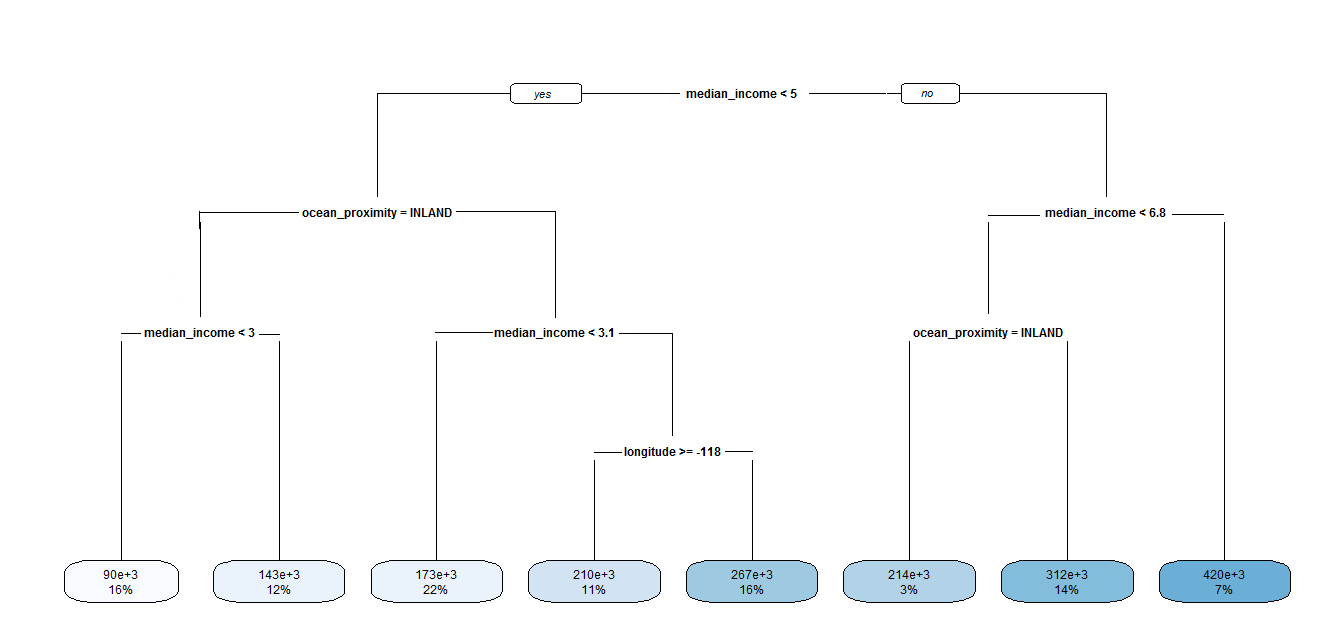
\includegraphics[width=9cm,height=8cm]{Images/cal-ID3.png}
\caption{\footnotesize{The ID3 decision tree. California Housing (Pace \& Barry, 1997).}}
\label{fig:cal_id3}
\end{figure}
\begin{figure}[h!]
\centering
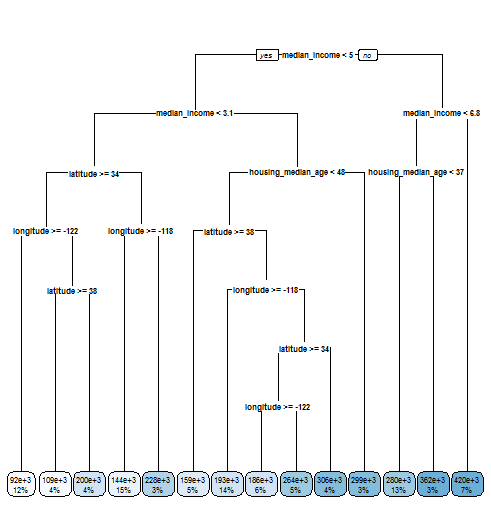
\includegraphics[width=9cm,height=8cm]{Images/cal-CCR.png}
\caption{\footnotesize{The CCRDT decision tree. California Housing (Pace \& Barry, 1997).}}
\label{fig:cal_ccrdt}
\end{figure}
\begin{figure}[h!]
\centering
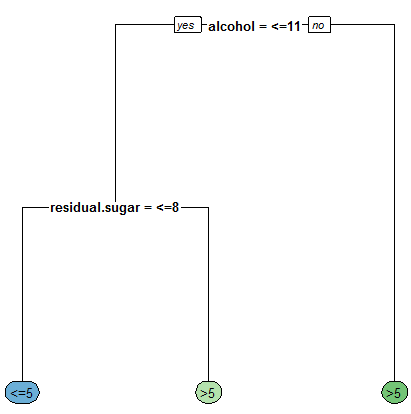
\includegraphics[width=6cm,height=4cm]{Images/win-ID3.png}
\caption{\footnotesize{The ID3 decision tree. Wine Quality (Cortez et al., 2009).}}
\label{fig:wine_id3}
\end{figure}
\begin{figure}[h!]
\centering
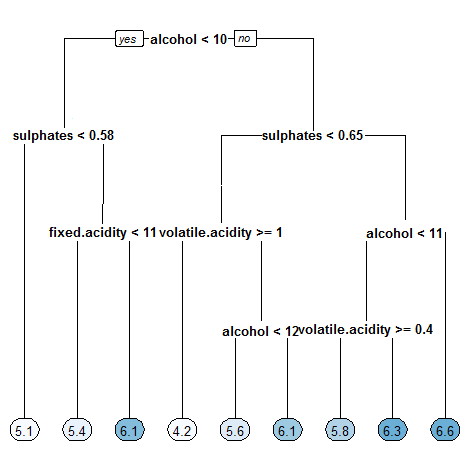
\includegraphics[width=9cm,height=8cm]{Images/win-CCR.png}
\caption{\footnotesize{The CCRDT decision tree. Wine Quality (Cortez et al., 2009).}}
\label{fig:wine_ccrdt}
\end{figure}
\begin{figure}[h!]
\centering
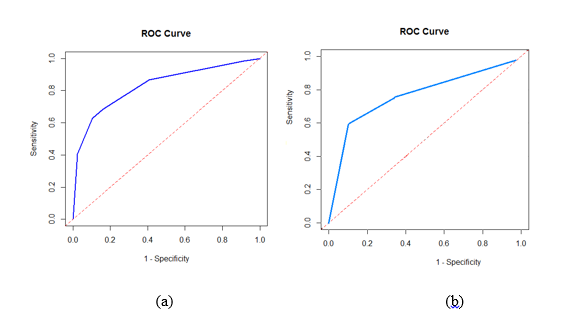
\includegraphics[width=8cm,height=5cm]{Images/ROC-cal.png}
\caption{\footnotesize{ROC curve of CCRDT (a) and ID3 (b) (California Housing).}}
\label{fig:roc_california}

\vspace{0.5cm}

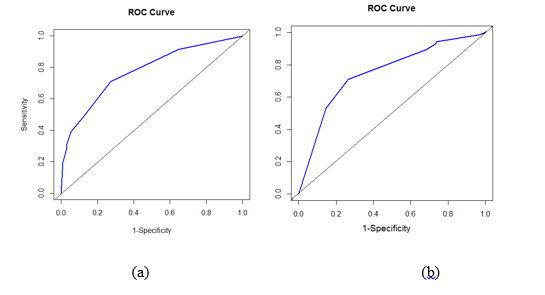
\includegraphics[width=8cm,height=5cm]{Images/ROC-win.png}
\caption{\footnotesize{ROC curve of CCRDT (a) and ID3 (b) (Wine Quality).}}
\label{fig:roc_wine}
\end{figure}
%\begin{figure}[ht]
%\begin{center}
%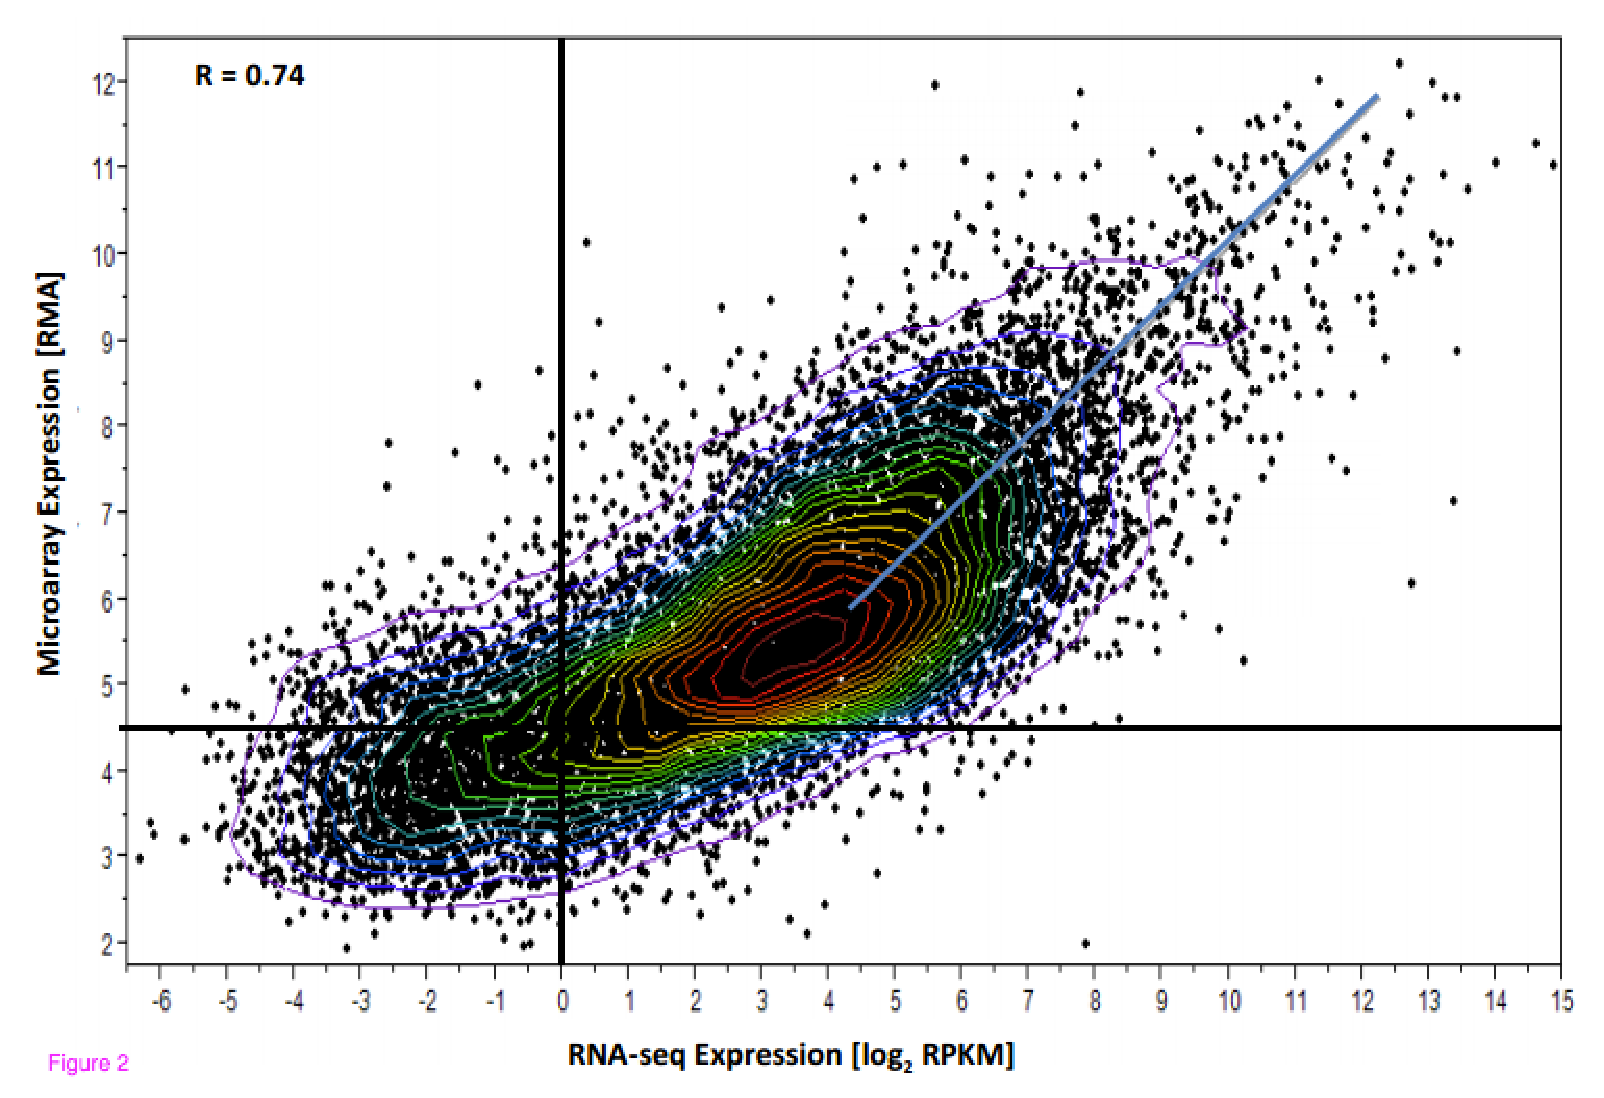
\includegraphics[width=7cm,height=6cm]{Images/Fig2.eps}
%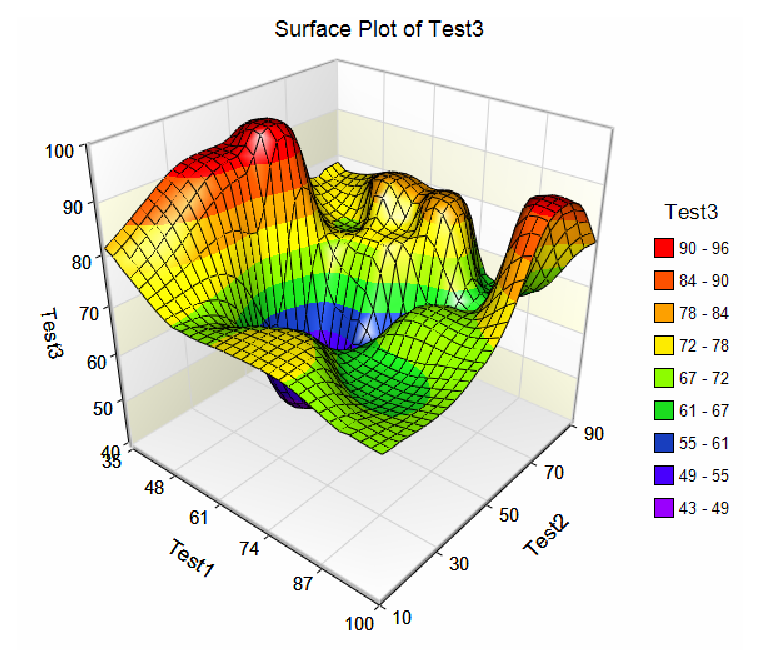
\includegraphics[width=7cm,height=6cm]{Images/Fig1.eps}\\
%\vspace{-0.2cm}
%\caption{\footnotesize{Figure caption should be placed here.}}\label{fig1}
%\end{center}
%\end{figure}
\section{Conclusion}

In contrast to conventional decision tree algorithms, the Conditional Cumulative Residual Decision Tree (CCRDT) eliminates the need for discretization by utilizing conditional cumulative residual entropy. This unique characteristic facilitates the development of decision trees that utilize the entirety of the information present in the dataset. As a result, the outcomes derived from CCRDT more accurately reflect the genuine underlying relationships within the data, unhindered by the limitations imposed by discretization.
%%%%%%%%%%%%%%%%%%%%%%%% Definition %%%%%%%%%%%%%%%%%%%%%%%%%%%%%%%%%%%
%\begin{dfn}\label{df1}
%This is a definition.
%\end{dfn}
%%%%%%%%%%%%%%%%%%%%%%%% Example %%%%%%%%%%%%%%%%%%%%%%%%%%%%%%%%%%%
%\begin{eg}\label{ex1}
%This is an example.
%\end{eg} 
%%%%%%%%%%%%%%%%%%%%%%%% Lemma %%%%%%%%%%%%%%%%%%%%%%%%%%%%%%%%%%%
%\begin{lem}\label{lm1}
%This is a lemma.
%\end{lem}
%%%%%%%%%%%%%%%%%%%%%%%% Theorem and proof  %%%%%%%%%%%%%%%%%%%%%%%%%%%%%%%%%%%
%\begin{thm}\label{th1}
%This is a theorem.
%\end{thm}
%\begin{proof}
%This is a proof. 
%\end{proof}
%%%%%%%%%%%%%%%%%%%%%%%%  Proposition  %%%%%%%%%%%%%%%%%%%%%%%%%%%%%%%%%%%
%\begin{pro}\label{pr1}
%This is a proposition.
%\end{pro}
%%%%%%%%%%%%%%%%%%%%%%%% Corollary %%%%%%%%%%%%%%%%%%%%%%%%%%%%%%%%%%%
%\begin{cor}\label{cor1}
%This is a corollary.
%\end{cor}
%%%%%%%%%%%%%%%%%%%%%%%% Remark %%%%%%%%%%%%%%%%%%%%%%%%%%%%%%%%%%%
%\begin{rem}\label{rm1}
%You can refer to definition \ref{df1}, lemma \ref{lm1}, theorem \ref{th1}, proposition \ref{pr1}, and
%corollary \ref{cor1} in the text.
%\end{rem}
%%%%%%%%%%%%%%%%%%%%%%%% Algorithm %%%%%%%%%%%%%%%%%%%%%%%%%%%%%%%%%%%
%\begin{alg}\label{alg1}
%This algorithm has the following \footnote{Steps}steps:
%\begin{itemize}
%\item 
%Step 1
%\item
%Step 2
%\item
%Step 3
%\end{itemize}
%\end{alg}
%\section{Formulas}
%%%%%%%%%%%%%%%%%%%%%%%%%%%%%%%% Unnumbered formula %%%%%%%%%%%%%%%%%%%%%%%
%A sample unnumbered formula is given below:
%\begin{equation*}
%\max\limits_{x \in \mathbb{R}} \ f(x).
%\end{equation*}
%%%%%%%%%%%%%%%%%%%%%%%%%%%%%%%% Numbered formula %%%%%%%%%%%%%%%%%%%%%%%
%Here is a sample of a numbered formula: 
%\begin{equation}\label{eq1}
%G_F(x)=\frac{1}{B(\alpha,\beta)}\int_{0}^{F(x)} t^{\alpha-1}(1-t)^{\beta-1}\,dt, \qquad \alpha>0, \beta>0.
%\end{equation}
%Formula numbering should be based on sections, and only relationships that are referenced in the text should have numbers.
%Below is a multiline formula that is the derivative of equation \eqref{eq1}:
%\begin{align}
%g_F(x)&=\frac{d}{dx} G_F(x)\nonumber\\
%&=\frac{1}{B(\alpha,\beta)} f(x) \left(F(x)\right)^{\alpha -1} \left(\bar F(x)\right)^{\beta -1}.
%\end{align}
%\section{Tables and Figures}
%Below is a sample table. Table \ref{tab1} contains four rows and three columns.
%\begin{table}[h]
%\begin{center}
%\small
%\caption{Table title should be here.}\label{tab1}
%\begin{tabular}{|c|cc|}
%  \hline
%  Column One & Column Two & Column Three \\  \hline \hline
%  1 & 2 & 3 \\
%  4 & 5 & 6 \\
%  7 & 8 & 9 \\  \hline
%\end{tabular}
%\end{center}
%\end{table}\\
%%%%%%%%%%%%%%%%%%%%%%%%%%%%%%%% Figure %%%%%%%%%%%%%%%%%%%%%%%%%%%%%%%%%
%Below is a sample figure. Figure \ref{fig1} contains two subfigures.
%\begin{figure}[ht]
%\begin{center}
%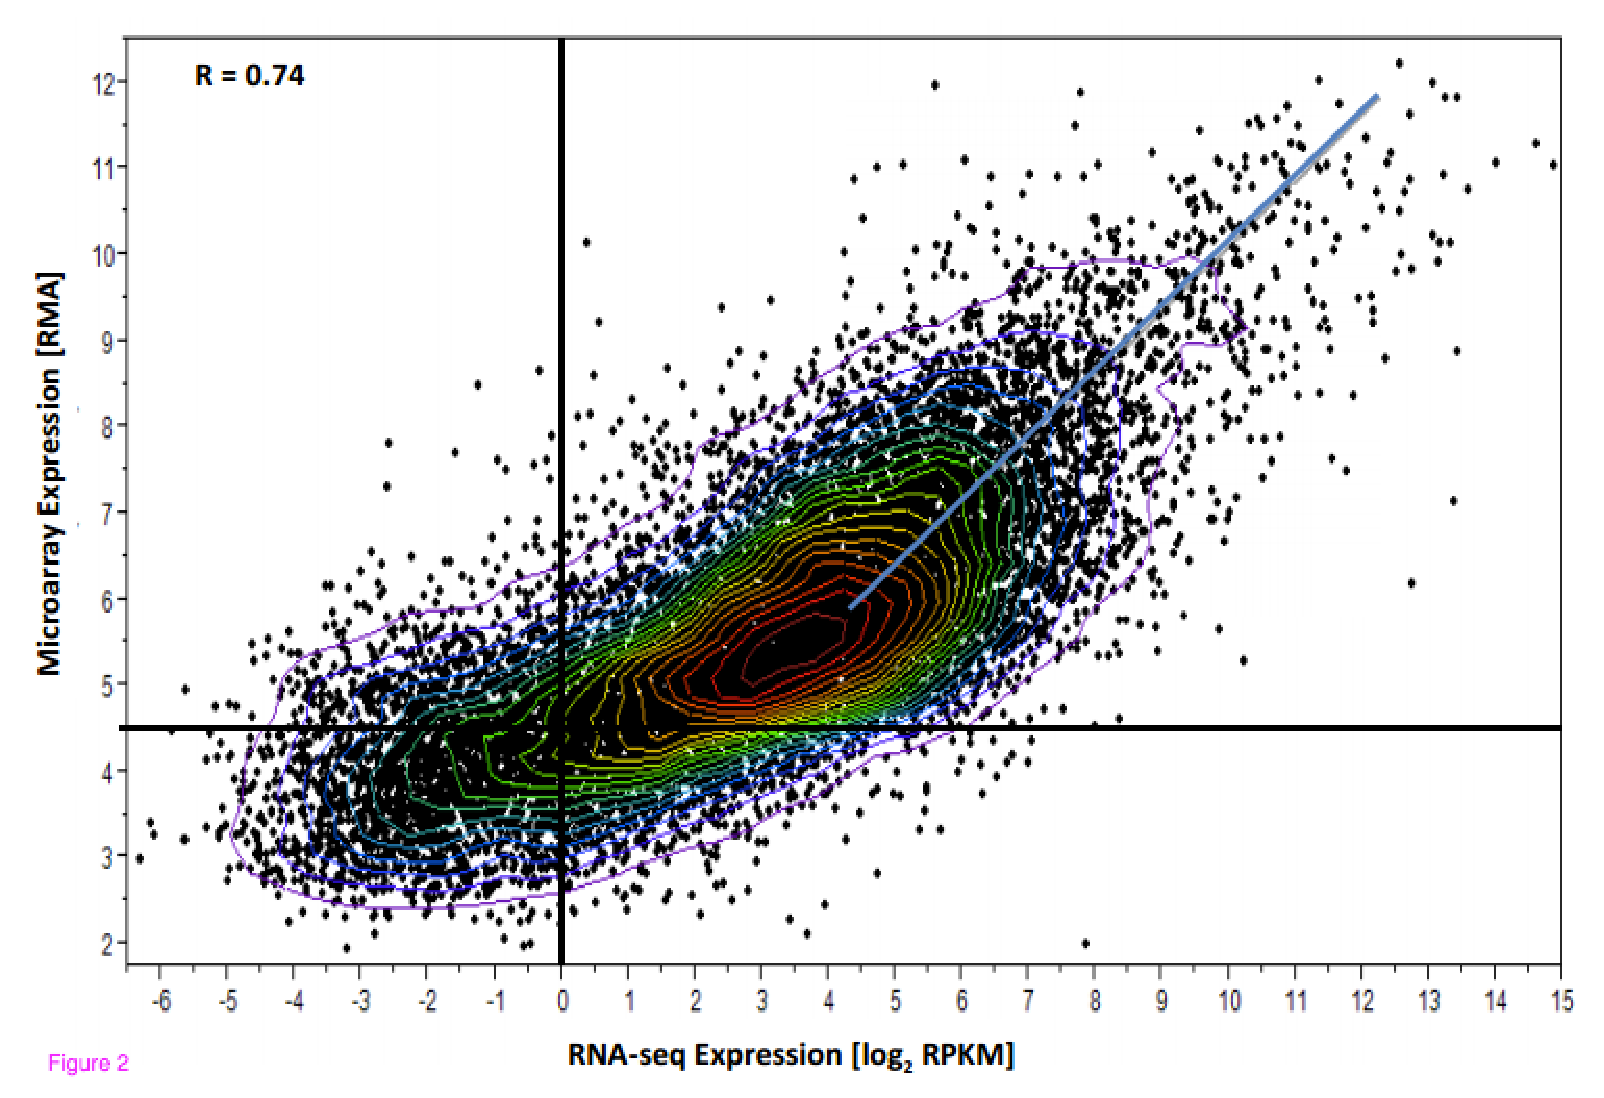
\includegraphics[width=7cm,height=6cm]{Images/Fig2.eps}
%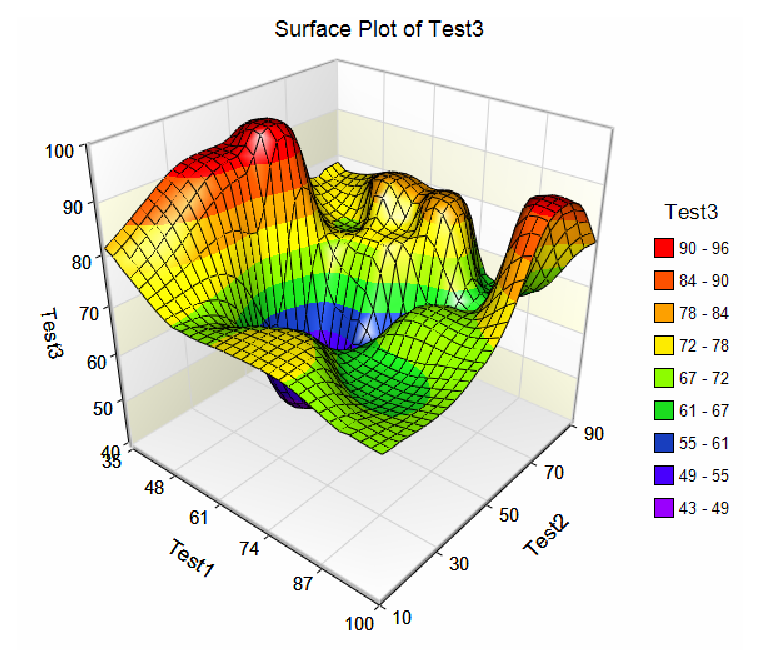
\includegraphics[width=7cm,height=6cm]{Images/Fig1.eps}\\
%\vspace{-0.2cm}
%\caption{\footnotesize{Figure caption should be placed here.}}\label{fig1}
%\end{center}
%\end{figure}
%%\section{Conclusion }
%%In contrast to conventional decision tree algorithms, the Conditional Cumulative Residual Decision Tree (CCRDT) eliminates the need for discretization by utilizing conditional cumulative residual entropy. This unique characteristic facilitates the development of decision trees that utilize the entirety of the information present in the dataset. As a result, the outcomes derived from CCRDT more accurately reflect the genuine underlying relationships within the data, unhindered by the limitations imposed by discretization. 
%\section*{Acknowledgments}   
%If you wish to include acknowledgments, this section should appear before the references.
%%%%%%%%%%%%%%%%%%%%%%%% References %%%%%%%%%%%%%%%%%%%%%%%%%%%%%
%
%\begin{thebibliography}{9}
%\bibitem[Craik (2005)]{Craik:2005}
%Craik A.D.D. (2005), Prehistory of Fa\`{a} di Bruno's formula, {\it The American Mathematical Monthly} 112, 2,  119-130.
%\bibitem[Feller (1972)]{Feller:1972} 
%Feller W. (1972), {\it An introduction to probability theory and its applications,} New York, John Wiley.
%\bibitem[Genest and  Rivest (1993)]{Genest:Rivest:1993}
%Genest C. and  Rivest L.P. (1993), Statistical inference
%procedures for bivariate Archimedean copulas, {\it J. Amer.
%Statist. Assoc.} 88,  1034 - 1043.
%
%\bibitem[Li et al. (2015)]{LZ15}
%Li K., Zheng W. and Ai M. (2015), Optimal designs for the proportional interference model, {\it The Annals of Statistics}, 43(4), 1596-1616.
\begin{thebibliography}{9}

\bibitem[Abolhossieni et al.(2024)]{Abolhossieni2024}
Abolhossieni, S. A., Khorashadizadeh, M., Chahkandi, M., \& Golalizadeh, M. (2024).
A modified ID3 decision tree algorithm based on cumulative residual entropy.
\emph{Expert Systems with Applications}, 124821.
http://dx.doi.org/10.2139/ssrn.4682847.

\bibitem[Brooks et al.(2014)]{Brooks2014}
Brooks, T., Pope, D., \& Marcolini, M. (2014).
Airfoil Self-Noise.
\emph{UCI Machine Learning Repository}.
https://doi.org/10.24432/C5VW2C.

\bibitem[Cortez \& Morais(2007)]{Cortez2007}
Cortez, P., \& Morais, A. D. J. R. (2007).
A data mining approach to predict forest fires using meteorological data.

\bibitem[Dong et al.(2022)]{Dong2022}
Dong, K., Li, S., \& Li, D. (2022).
Some properties of fractional cumulative residual entropy and fractional conditional cumulative residual entropy.
\emph{Fractal and Fractional}, 6(7), 400.
https://doi.org/10.3390/fractalfract6070400.

\bibitem[Han et al.(2012)]{Han2012}
Han, J., Kamber, M., \& Pei, J. (2012).
\emph{Data mining concepts and techniques} (3rd ed.).
University of Illinois at Urbana-Champaign.

\bibitem[Lasha Gochiashvili(2023)]{Lasha2023}
Lasha Gochiashvili. (2023).
Life Expectancy (WHO) Fixed.
\emph{Kaggle}.
https://doi.org/10.34740/KAGGLE/DS/3065197.

\bibitem[Meira-Machado \& Sestelo(2016)]{Meira2016}
Meira-Machado, L., \& Sestelo, M. (2016).
condSURV: An R Package for the Estimation of the Conditional Survival Function for Ordered Multivariate Failure Time Data.
\emph{R Journal}, 8(2), 460.
https://cran.r-project.org/web/packages/condSURV/.

\bibitem[Mirali et al.(2017)]{Mirali2017}
Mirali, M., Baratpour, S., \& Fakoor, V. (2017).
On weighted cumulative residual entropy.
\emph{Communications in Statistics - Theory and Methods}, 46(6), 2857-2869.
https://doi.org/10.1080/03610926.2015.1053932.

\bibitem[Nash et al.(1995)]{Nash1995}
Nash, W., Sellers, T., Talbot, S., Cawthorn, A., \& Ford, W. (1995).
Abalone.
\emph{UCI Machine Learning Repository}.
https://doi.org/10.24432/C55C7W.

\bibitem[Pace \& Barry(1997)]{Pace1997}
Pace, R. K., \& Barry, R. (1997).
Sparse spatial autoregressions.
\emph{Statistics \& Probability Letters}, 33(3), 291-297.
https://doi.org/10.1016/S0167-7152(96)00140-X.

\bibitem[Rajesh et al.(2016)]{Rajesh2016}
Rajesh, G., EI, A. S., KV, R., \& KR, M. N. (2016).
The conditional dynamic cumulative residual entropy.
\emph{Journal of the Japan Statistical Society}, 45(2), 99-119.
https://doi.org/10.14490/jjss.45.99.

\bibitem[Rao et al.(2004)]{Rao2004}
Rao, M., Chen, Y., Vemuri, B. C., \& Wang, F. (2004).
Cumulative residual entropy: a new measure of information.
\emph{IEEE Transactions on Information Theory}, 50(6), 1220-1228.
https://doi.org/10.1109/TIT.2004.828057.

\bibitem[Tsanas \& Xifara(2012)]{Tsanas2012}
Tsanas, A., \& Xifara, A. (2012).
Accurate quantitative estimation of energy performance of residential buildings using statistical machine learning tools.
\emph{Energy and Buildings}, 49, 560-567.
https://doi.org/10.24432/C51307.

\bibitem[T\"ufekci(2014)]{Tufekci2014}
Tüfekci, P. (2014).
Prediction of full load electrical power output of a base load operated combined cycle power plant using machine learning methods.
\emph{International Journal of Electrical Power \& Energy Systems}, 60, 126-140.
https://doi.org/10.24432/C5002N.

\bibitem[Yeh(1998)]{Yeh1998}
Yeh, I. C. (1998).
Modeling of strength of high-performance concrete using artificial neural networks.
\emph{Cement and Concrete Research}, 28(12), 1797-1808.

\bibitem[Craik(2005)]{Craik2005}
Craik, A. D. D. (2005).
Prehistory of Fa\`a di Bruno's formula.
\emph{The American Mathematical Monthly}, 112(2), 119-130.

\end{thebibliography}
 \end{document}

